\chapter{Applications conformes et prescription de diffusion des cordes ouvertes}

\lectureoverview{Les applications conformes apparaissent d’abord comme une symétrie pratique de l’électrostatique bidimensionnelle. La différentiabilité complexe rend cette symétrie calculable : les équations de Cauchy--Riemann impliquent l’équation de Laplace, et une dérivée complexe indépendante de la direction préserve les angles. Grâce à ces outils, on peut représenter la surface d’univers d’une corde sous la forme d’une bande, d’un demi-plan, d’un cylindre ou d’un disque sans modifier la physique. La diffusion des cordes ouvertes se ramène alors à une intégrale de chemin gaussienne sur le disque, avec des insertions de quantité de mouvement sur son bord, suivie d’une intégration sur leurs positions non équivalentes.}

\section{Électrostatique dans un monde bidimensionnel}

Commençons par un problème d’électrostatique strictement bidimensionnel. Les charges et leurs lignes de champ sont confinées à un plan ; il ne s’agit pas simplement de charges ordinaires tridimensionnelles dont le mouvement se ferait dans un plan. La loi de Gauss donne alors
\begin{equation}
  F(r)\propto \frac{1}{r},
  \qquad
  V(r)\propto \log r,
  \label{eq:l08-two-dimensional-coulomb}
\end{equation}
car le flux traverse un cercle dont la circonférence croît comme \(r\).

Écrivons le champ à l’aide d’un potentiel scalaire \(\phi\). Avec la convention de signe utilisée au tableau,
\begin{equation}
  \mathbf E=\nabla\phi,
  \qquad
  \nabla\cdot\mathbf E=\rho,
\end{equation}
et donc
\begin{equation}
  \nabla^2\phi
  =\frac{\partial^2\phi}{\partial x^2}
  +\frac{\partial^2\phi}{\partial y^2}
  =\rho.
  \label{eq:l08-poisson}
\end{equation}
Dans une région sans charge, cela se réduit à l’équation de Laplace,
\begin{equation}
  \nabla^2\phi=0.
  \label{eq:l08-laplace-phi}
\end{equation}
\editorialnote{De nombreux textes d’électrodynamique définissent
\(\mathbf E=-\nabla\Phi\), auquel cas
\(\nabla^2\Phi=-\rho\) après absorption des constantes. Dans ce cours, le signe du potentiel est choisi à l’opposé. L’équation sans source et tous les arguments conformes restent inchangés.}

\begin{figure}[H]
  \centering
  \includegraphics[width=0.72\textwidth]{lecture_08_figure_01.png}
  \caption{Les équations de l’électrostatique mises sous la forme de l’opérateur de Poisson bidimensionnel.}
  \lectureframe{00:03:48}
  \label{fig:l08-electrostatics-board}
\end{figure}

Le signe plus entre les deux dérivées spatiales est essentiel. Il fait de cette équation une équation elliptique, et non une équation d’onde. Les transformations conformes préservent sa forme sans source : une solution sur un domaine peut donc être transportée vers un domaine de forme différente, avec ses conditions aux limites. Cette propriété est utile en électrostatique, en mécanique des fluides bidimensionnelle et en cartographie, avant de l’être en théorie des cordes.

\begin{classroomqa}
\audiencequestion{Si le laplacien s’annule, s’agit-il d’une équation d’onde stationnaire ? \lecturetimestamp{00:05:35}}
\lecturerresponse{Non. Les deux dérivées spatiales ont le même signe, et il n’y a pas de dérivée temporelle. Une équation d’onde exige une dépendance temporelle avec le signe relatif lorentzien. L’électrostatique est précisément statique : rien n’évolue, pas même une onde.}
\end{classroomqa}

\begin{classroomqa}
\audiencequestion{Existe-t-il un rotationnel en deux dimensions ?
\lecturetimestamp{00:06:06}}
\lecturerresponse{Oui, mais il n’a qu’une seule composante indépendante. Pour
\(\mathbf E=(E_x,E_y)\),
\[
  \operatorname{curl}_{2d}\mathbf E
  =\partial_yE_x-\partial_xE_y.
\]
On peut se le représenter comme la composante perpendiculaire au tableau, même si un monde intrinsèquement bidimensionnel n’a pas besoin d’une direction perpendiculaire extérieure. En dimension supérieure, l’objet correspondant est naturellement une 2-forme antisymétrique.}
\end{classroomqa}

\section{Une dérivée sans direction privilégiée}

Introduisons des coordonnées complexes dans les plans de départ et d’arrivée :
\begin{equation}
  z=x+iy,
  \qquad
  w=u+iv,
  \qquad
  w=w(z).
  \label{eq:l08-complex-coordinates}
\end{equation}
Ici, \(x,y,u,v\) sont réels. Localement, la dérivée devrait être
\begin{equation}
  \frac{dw}{dz}
  =\lim_{\Delta z\to0}\frac{\Delta w}{\Delta z}.
  \label{eq:l08-complex-derivative}
\end{equation}
Contrairement à la droite réelle, le plan complexe admet une infinité de directions d’approche. Une application continue et, en général, régulière ne donne pas nécessairement le même rapport dans toutes ces directions.

Comparons deux approches simples. Dans la direction \(x\), \(dy=0\), donc
\begin{equation}
  \left.\frac{dw}{dz}\right|_x
  =\frac{\partial u}{\partial x}
  +i\frac{\partial v}{\partial x}.
\end{equation}
Dans la direction \(y\), \(dx=0\), et
\begin{equation}
  \left.\frac{dw}{dz}\right|_y
  =\frac{1}{i}\frac{\partial u}{\partial y}
  +\frac{\partial v}{\partial y}
  =\frac{\partial v}{\partial y}
  -i\frac{\partial u}{\partial y}.
\end{equation}
L’égalité des parties réelle et imaginaire donne
\begin{equation}
  \boxed{
  \frac{\partial u}{\partial x}
  =\frac{\partial v}{\partial y},
  \qquad
  \frac{\partial u}{\partial y}
  =-\frac{\partial v}{\partial x}}
  \label{eq:l08-cauchy-riemann}
\end{equation}
Ce sont les équations de Cauchy--Riemann. Sous les hypothèses usuelles de différentiabilité, elles suffisent aussi à garantir que la limite
\eqref{eq:l08-complex-derivative} est indépendante de la direction. Une fonction qui possède cette propriété est dite analytique, ou holomorphe, au point considéré.

\begin{figure}[H]
  \centering
  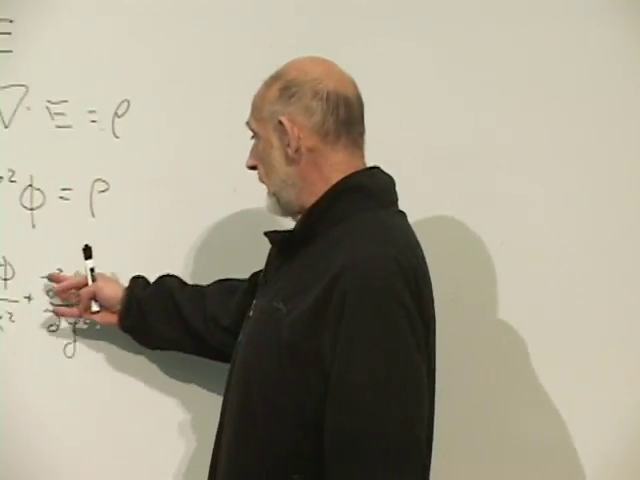
\includegraphics[width=0.70\textwidth]{lecture_08_figure_02.png}
  \caption{Le système complet de Cauchy--Riemann, avec le signe moins relatif.}
  \lectureframe{00:19:48}
  \label{fig:l08-cr-board}
\end{figure}

Le cours distingue brièvement des termes apparentés. Une fonction holomorphe sur tout le plan complexe fini est dite entière. Une fonction méromorphe peut avoir des pôles isolés. Ainsi, \(1/z\) est analytique sauf en \(z=0\), mais n’est pas entière.

\section{Conjuguées harmoniques et géométrie conforme}

Les équations de Cauchy--Riemann sont des équations couplées du premier ordre, mais elles impliquent des équations distinctes du second ordre. Dérivons
\(\partial_xu=\partial_yv\) par rapport à \(x\), dérivons
\(\partial_yu=-\partial_xv\) par rapport à \(y\), puis additionnons :
\begin{align}
  \partial_x^2u&=\partial_x\partial_yv,\\
  \partial_y^2u&=-\partial_y\partial_xv,\\
  \therefore\qquad
  \partial_x^2u+\partial_y^2u&=0.
  \label{eq:l08-harmonic-u}
\end{align}
En répétant le raisonnement en échangeant \(u\) et \(v\), on obtient
\begin{equation}
  \partial_x^2v+\partial_y^2v=0.
  \label{eq:l08-harmonic-v}
\end{equation}
Les parties réelle et imaginaire d’une fonction analytique sont donc des conjuguées harmoniques. Deux fonctions harmoniques quelconques ne définissent pas automatiquement une fonction analytique : elles doivent encore être liées par
\eqref{eq:l08-cauchy-riemann}.

\begin{figure}[H]
  \centering
  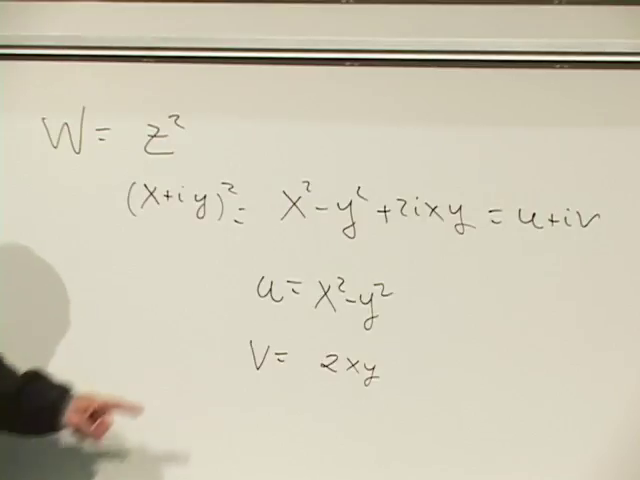
\includegraphics[width=0.68\textwidth]{lecture_08_figure_03.png}
  \caption{Les dérivées mixtes s’annulent ; il reste l’équation de Laplace pour une composante de l’application analytique.}
  \lectureframe{00:23:09}
  \label{fig:l08-harmonic-board}
\end{figure}

On peut aussi donner une interprétation vectorielle. Si
\(\mathbf F=(u,-v)\), les deux équations de Cauchy--Riemann expriment, à un choix d’orientation près, que la divergence et le rotationnel bidimensionnel de \(\mathbf F\) sont tous deux nuls. Nous voici donc revenus à l’électrostatique.

\subsection{Pourquoi les angles sont préservés}

Écrivons deux petits déplacements complexes sous forme polaire :
\begin{equation}
  \delta z=\rho e^{i\theta},
  \qquad
  \Delta z=\rho'e^{i\theta'}.
\end{equation}
La phase de leur rapport est \(\theta-\theta'\), exactement l’angle entre eux. Sous une application analytique,
\begin{equation}
  \frac{\delta w}{\delta z}
  =\frac{\Delta w}{\Delta z}
  =w'(z),
\end{equation}
car la dérivée ne dépend pas de la direction. En réarrangeant, on obtient
\begin{equation}
  \frac{\Delta z}{\delta z}
  =\frac{\Delta w}{\delta w}.
  \label{eq:l08-angle-ratio}
\end{equation}
Les deux membres ont la même phase ; l’angle entre les intervalles initiaux est donc égal à celui entre leurs images.

\begin{figure}[H]
  \centering
  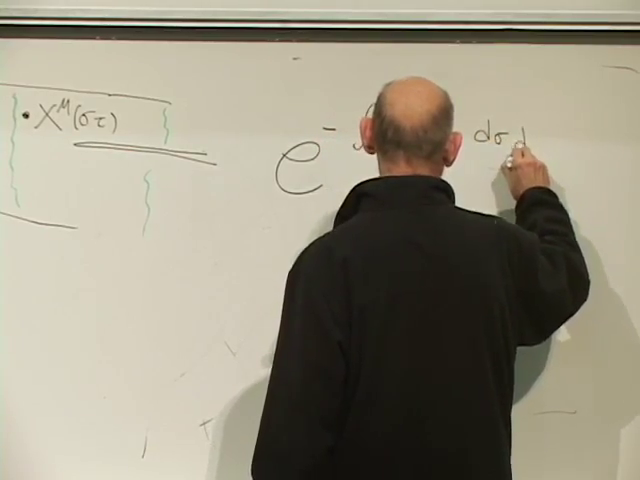
\includegraphics[width=0.70\textwidth]{lecture_08_figure_04.png}
  \medskip

  \begin{tikzpicture}[x=0.9cm,y=0.9cm,>=Latex]
    \begin{scope}
      \draw[->] (-0.2,0) -- (2.3,0);
      \draw[->] (0,-0.2) -- (0,2.1);
      \draw[very thick,blue!65!black,->] (0,0) -- (1.85,0.45)
        node[right] {\(\delta z\)};
      \draw[very thick,orange!75!black,->] (0,0) -- (0.72,1.65)
        node[above] {\(\Delta z\)};
      \draw (0.58,0.14) arc[start angle=14,end angle=66,radius=0.60];
      \node at (1.0,-0.55) {\(z\)-plane};
    \end{scope}
    \draw[->,thick] (3.0,0.9) -- (4.2,0.9)
      node[midway,above] {\(w(z)\)};
    \begin{scope}[xshift=5.0cm]
      \draw[->] (-0.2,0) -- (2.3,0);
      \draw[->] (0,-0.2) -- (0,2.1);
      \draw[very thick,blue!65!black,->] (0,0) -- (1.65,0.70)
        node[right] {\(\delta w\)};
      \draw[very thick,orange!75!black,->] (0,0) -- (0.48,1.62)
        node[above] {\(\Delta w\)};
      \draw (0.54,0.23) arc[start angle=23,end angle=74,radius=0.59];
      \node at (1.0,-0.55) {\(w\)-plane};
    \end{scope}
  \end{tikzpicture}
  \caption{La démonstration au tableau et une reconstruction locale claire. La multiplication par \(w'(z)\) fait tourner et change d’échelle chaque direction infinitésimale de la même façon, préservant ainsi leur angle relatif.}
  \lectureframe{00:34:11}
  \label{fig:l08-angle-proof}
\end{figure}

Ce raisonnement local suppose que \(w'(z)\neq0\). En un point critique, l’application peut ne pas être localement bijective, et la géométrie doit être étudiée séparément. En dehors de ces points, les applications analytiques et les applications conformes qui préservent l’orientation sont localement les mêmes.

\section{Quelques exemples pour exercer l’œil}

\subsection{Carré et conjugaison complexe}

Pour \(w=z^2\),
\begin{equation}
  (x+iy)^2=x^2-y^2+2ixy=u+iv,
\end{equation}
donc
\begin{equation}
  u=x^2-y^2,
  \qquad
  v=2xy.
  \label{eq:l08-z-squared-components}
\end{equation}
Les dérivées secondes de \(u\) sont \(2\) et \(-2\) ; celles de \(v\) s’annulent séparément. Les deux fonctions sont harmoniques, et une dérivation directe vérifie également les équations de Cauchy--Riemann.

\begin{figure}[H]
  \centering
  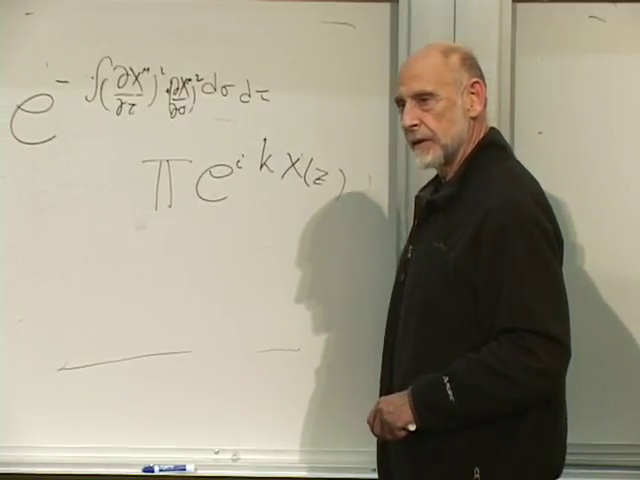
\includegraphics[width=0.72\textwidth]{lecture_08_figure_05.png}
  \caption{L’application qui élève au carré, décomposée en ses composantes harmoniques réelle et imaginaire.}
  \lectureframe{00:36:45}
  \label{fig:l08-z-square-board}
\end{figure}

\begin{classroomqa}
\audiencequestion{La fonction \(1/z\) fournit-elle un exemple non analytique ?
\lecturetimestamp{00:37:49}}
\lecturerresponse{En un seul point. Elle est analytique partout où \(z\neq0\) et possède un pôle à l’origine. Pour voir une application qui échoue partout au test de Cauchy--Riemann, la conjugaison complexe est un meilleur exemple.}
\end{classroomqa}

En revanche,
\begin{equation}
  w=\bar z=x-iy
  \qquad\Longrightarrow\qquad
  u=x,\quad v=-y
\end{equation}
inverse l’orientation. Ses dérivées ne satisfont pas la première équation de Cauchy--Riemann, à cause d’un signe ; cette fonction de \(z\) n’est donc pas analytique.

\begin{figure}[H]
  \centering
  \includegraphics[width=0.62\textwidth]{lecture_08_figure_06.png}
  \caption{La conjugaison complexe constitue le contre-exemple délibérément non analytique.}
  \lectureframe{00:38:38}
  \label{fig:l08-conjugate-board}
\end{figure}

\subsection{L’exponentielle et sa réciproque}

\begin{classroomqa}
\audiencequestion{Si \(e^z\) est analytique, pourquoi son inverse \(\log z\) le serait-elle aussi ? \lecturetimestamp{00:40:38}}
\lecturerresponse{Lorsque l’inverse existe et que \(w'(z)\neq0\), sa dérivée vaut \(1/w'(z)\). L’indépendance par rapport à la direction est donc préservée. À l’échelle globale, le logarithme est multivalué ; on choisit donc une branche et on exclut son point de branchement et sa coupure. L’énoncé conforme local reste valable sur le domaine ainsi choisi.}
\end{classroomqa}

La formule d’Euler donne
\begin{equation}
  w=e^z=e^{x+iy}
  =e^x(\cos y+i\sin y),
\end{equation}
d’où
\begin{equation}
  u=e^x\cos y,
  \qquad
  v=e^x\sin y.
  \label{eq:l08-exponential-components}
\end{equation}
Par exemple,
\(\partial_xu=e^x\cos y=\partial_yv\), et la seconde équation de Cauchy--Riemann se vérifie tout aussi directement.

\begin{figure}[H]
  \centering
  \includegraphics[width=0.68\textwidth]{lecture_08_figure_07.png}
  \caption{Les composantes réelle et imaginaire de l’application exponentielle.}
  \lectureframe{00:42:23}
  \label{fig:l08-exponential-board}
\end{figure}

\section{Demi-plan, bande, cylindre et disque}

\subsection{Le logarithme transforme le rayon en temps}

Considérons le demi-plan droit, où
\(-\pi/2<\theta<\pi/2\), et écrivons
\begin{equation}
  z=re^{i\theta},
  \qquad
  w=\log z=\log r+i\theta.
  \label{eq:l08-log-map}
\end{equation}
Le demi-plan est envoyé sur la bande infinie
\begin{equation}
  -\frac{\pi}{2}<\operatorname{Im}w<\frac{\pi}{2}.
\end{equation}
Les demi-droites de \(\theta\) constant deviennent des droites horizontales, tandis que les demi-cercles de \(r\) constant deviennent des droites verticales. L’origine est envoyée sur \(\operatorname{Re}w=-\infty\), et \(r=\infty\) sur \(\operatorname{Re}w=+\infty\).

\begin{figure}[H]
  \centering
  \includegraphics[width=0.75\textwidth]{lecture_08_figure_08.png}
  \caption{Le logarithme envoie le demi-plan droit sur une bande infinie : les demi-droites polaires et les demi-cercles deviennent une grille rectangulaire orthogonale.}
  \lectureframe{00:47:48}
  \label{fig:l08-log-strip-board}
\end{figure}

La bande est la surface d’univers standard d’une corde ouverte. Sa coordonnée bornée paramètre la position le long de la corde, tandis que la translation dans la direction non bornée correspond au temps de la surface d’univers. Par l’application exponentielle inverse, une translation dans le temps devient une dilatation \(z\mapsto e^a z\). Ainsi, la même symétrie prend la forme d’une translation dans la bande et d’une expansion uniforme dans le demi-plan.

\begin{classroomqa}
\audiencequestion{Où va un point particulier, par exemple \(r=1\), et les coordonnées de la bande sont-elles encore polaires ? \lecturetimestamp{00:50:58}}
\lecturerresponse{Un cercle de rayon fixe devient une droite verticale en \(\operatorname{Re}w=\log r\) ; en particulier, \(r=1\) est envoyé sur la droite centrale \(\operatorname{Re}w=0\). Les coordonnées polaires décrivent le plan \(z\). Le plan \(w\) utilise des coordonnées cartésiennes ordinaires \((\log r,\theta)\).}
\end{classroomqa}

Si l’on applique \(\log z\) au plan privé de l’origine tout entier, la coordonnée angulaire est périodique de \(2\pi\). La bande obtenue a donc ses bords supérieur et inférieur identifiés : c’est un cylindre infini. Le demi-plan avec son bord décrit la surface d’univers d’une corde ouverte ; le plan entier, sans bord et avec un angle périodique, décrit un cylindre de corde fermée.

\begin{figure}[H]
  \centering
  \includegraphics[width=0.75\textwidth]{lecture_08_figure_09.png}
  \caption{La représentation du demi-plan en bande et l’identification périodique qui transforme le plan privé de l’origine en un cylindre de corde fermée.}
  \lectureframe{00:54:23}
  \label{fig:l08-open-closed-board}
\end{figure}

\subsection{Une application de Cayley vers le disque unité}

Une transformation homographique, ou transformation de Möbius, envoie le demi-plan droit sur le disque unité :
\begin{equation}
  w=\frac{z-1}{z+1}.
  \label{eq:l08-cayley}
\end{equation}
Elle envoie \(z=0\) sur \(-1\), \(z=\infty\) sur \(+1\), et l’axe imaginaire sur \(|w|=1\). Si \(z=ir\),
\begin{equation}
  \left|\frac{ir-1}{ir+1}\right|=1.
\end{equation}
Les points tels que \(\operatorname{Re}z>0\) se trouvent à l’intérieur du cercle ; le demi-plan gauche est envoyé à l’extérieur.
\editorialnote{Lors de la dérivation au tableau, on écrit l’inverse \((z+1)/(z-1)\) alors qu’on décrit l’image intérieure du disque. Cet inverse a le même cercle unité pour frontière, mais envoie le demi-plan droit à l’extérieur. L’équation \eqref{eq:l08-cayley} correspond à la convention de l’intérieur du disque, cohérente avec la géométrie énoncée.}

\begin{figure}[H]
  \centering
  \includegraphics[width=0.72\textwidth]{lecture_08_figure_10.png}
  \caption{Construction homographique de la frontière du cercle unité. La convention réciproque visible au tableau échange l’intérieur et l’extérieur.}
  \lectureframe{00:58:38}
  \label{fig:l08-cayley-board}
\end{figure}

Les transformations de Möbius envoient l’ensemble généralisé des cercles et des droites sur des cercles et des droites. La grille radiale et circulaire du demi-plan devient donc deux familles orthogonales d’arcs dans le disque. Un diamètre droit est simplement le cas limite d’un cercle dont le centre est rejeté à l’infini.

\begin{classroomqa}
\audiencequestion{Les arcs tracés à l’intérieur du disque sont-ils vraiment des cercles ?
\lecturetimestamp{01:00:55}}
\lecturerresponse{Oui. Leurs centres se trouvent à des endroits différents, souvent à l’extérieur du disque visible. Le diamètre est la limite de rayon infini de cette même famille.}
\end{classroomqa}

\begin{classroomqa}
\audiencequestion{Le dessin du disque signifie-t-il qu’il s’agit d’une sphère, et où va l’autre demi-plan ? \lecturetimestamp{01:01:21}}
\lecturerresponse{Le dessin présenté ici est un disque plat, pas une sphère. Le demi-plan droit est envoyé à l’intérieur de son bord et le demi-plan gauche à l’extérieur. Si l’on ajoute le point à l’infini au plan complexe tout entier, ce plan étendu peut être représenté par une sphère au moyen d’une projection stéréographique ; c’est un énoncé global différent.}
\end{classroomqa}

\begin{classroomqa}
\audiencequestion{Quelles courbes du disque correspondent aux rayons et aux demi-cercles de rayon constant du plan initial ? \lecturetimestamp{01:02:59}}
\lecturerresponse{L’axe réel positif devient le diamètre reliant \(-1\) et \(+1\). Les autres demi-droites deviennent des arcs de cercle reliant ces mêmes points du bord. Les demi-cercles de rayon fixe deviennent la famille orthogonale qui rejoint le cercle unité en deux points.}
\end{classroomqa}

\begin{figure}[H]
  \centering
  \includegraphics[width=0.72\textwidth]{lecture_08_figure_11.png}
  \caption{Dans le demi-plan, les droites et les demi-cercles deviennent dans le disque des familles orthogonales de cercles et de droites.}
  \lectureframe{01:03:48}
  \label{fig:l08-circle-grid-board}
\end{figure}

\section{La surface d’univers à quatre cordes}

Nous pouvons maintenant revenir à la diffusion. Deux cordes ouvertes entrent, s’unissent en une seule, se propagent pendant un intervalle quelconque, puis se séparent en deux cordes sortantes. En coordonnées de bande, la surface d’univers ressemble à un long ruban fendu à chaque extrémité---— l’image du « pansement sportif ». La durée de vie de l’état intermédiaire n’est pas fixée à l’avance. Elle fait partie des histoires sur lesquelles on intègre l’amplitude.

Soient \((\sigma,\tau)\) les coordonnées sur la surface d’univers, et soit
\begin{equation}
  X^\mu=X^\mu(\sigma,\tau)
  \label{eq:l08-embedding}
\end{equation}
sa position dans l’espace-temps. Les indices \(\sigma,\tau\) désignent les coordonnées sur la surface paramétrique bidimensionnelle ; l’indice \(\mu\) désigne les coordonnées d’espace-temps. Dans la théorie bosonique, \(\mu=0,\ldots,25\) ; dans le cas des supercordes, l’espace-temps compte dix coordonnées.

Après rotation de Wick, les champs d’immersion libres ont pour action euclidienne
\begin{equation}
  S_E[X]
  =\frac{1}{4\pi\alpha'}\int_\Sigma d\sigma\,d\tau\,
  \left[
    \partial_\tau X^\mu\partial_\tau X_\mu
    +\partial_\sigma X^\mu\partial_\sigma X_\mu
  \right].
  \label{eq:l08-euclidean-action}
\end{equation}
L’intégrale de chemin correspondante somme sur toutes les immersions de la surface d’univers choisie dans l’espace-temps :
\begin{equation}
  \int\mathcal D X\,e^{-S_E[X]}.
  \label{eq:l08-bare-worldsheet-integral}
\end{equation}

\begin{figure}[H]
  \centering
  \includegraphics[width=0.74\textwidth]{lecture_08_figure_12.png}
  \caption{Le poids euclidien positif complet de la surface d’univers. Les deux termes en dérivées sont sommés sur toutes les composantes d’espace-temps.}
  \lectureframe{01:11:34}
  \label{fig:l08-action-board}
\end{figure}

La bande fendue possède un bord connexe. La liberté conforme permet donc de la représenter par un disque. Les quatre extrémités éloignées des bandes deviennent quatre points marqués sur le bord. Déplacer ces points modifie la séparation apparente entre la réunion et la séparation dans les coordonnées de bande, mais ne change ni la surface sous-jacente ni la physique.

\begin{figure}[H]
  \centering
  \includegraphics[width=0.76\textwidth]{lecture_08_figure_13.png}
  \caption{La surface d’univers en bande fendue et sa représentation sur un disque, avec les points du bord associés aux cordes externes.}
  \lectureframe{01:15:18}
  \label{fig:l08-bandage-disc-board}
\end{figure}

Les lignes de la grille détaillée utilisées pour représenter cette application conforme n’ont pas de signification physique. Ce qui importe, c’est la topologie, le bord et les points externes marqués. On peut étirer la même surface d’univers pour obtenir différentes représentations selon le canal, sans introduire de nouvelle interaction.

\section{États externes sous forme d’insertions au bord}

L’intégrale sans insertions \eqref{eq:l08-bare-worldsheet-integral} n’indique pas encore quelles quantités de mouvement entrent et sortent. Pour un état scalaire de corde ouverte de quantité de mouvement \(k_i^\mu\), insérons sur le bord l’opérateur vertex
\begin{equation}
  V_i(z_i)=e^{\,i k_i\cdot X(z_i)},
  \qquad
  k_i\cdot X=k_{i\mu}X^\mu.
  \label{eq:l08-vertex}
\end{equation}
Le point \(z_i\) est une position sur le bord de la surface d’univers. Ce n’est ni une coordonnée d’espace-temps ni une direction de quantité de mouvement.

\begin{figure}[H]
  \centering
  \includegraphics[width=0.72\textwidth]{lecture_08_figure_14.png}
  \caption{Le poids euclidien dans le volume et le produit des insertions de quantité de mouvement au bord sont représentés comme des facteurs distincts.}
  \lectureframe{01:18:58}
  \label{fig:l08-vertex-board}
\end{figure}

Pour \(n\) cordes ouvertes externes, la prescription schématique est
\begin{equation}
  \begin{aligned}
    \mathcal A_n(k_1,\ldots,k_n)
    &=\int_{\mathcal M_{0,n}^{\partial}}\!d\mu(z_i)
      \int\mathcal D X\\
    &\quad\times e^{-S_E[X]}
      \prod_{i=1}^{n}e^{\,i k_i\cdot X(z_i)}.
  \end{aligned}
  \label{eq:l08-open-string-prescription}
\end{equation}
L’intégrale fonctionnelle porte sur les immersions \(X^\mu\). L’intégrale de dimension finie porte sur les positions d’insertion non équivalentes au bord. À ce stade, les facteurs de polarisation et la mesure de fixation de jauge sont omis, comme dans le cours.
\editorialnote{Une amplitude de corde complètement fixée en jauge comprend également la contribution de fantômes appropriée, les facteurs de vertex dépendant de l’état, les constantes de couplage et la normalisation. L’équation
\eqref{eq:l08-open-string-prescription} décrit la dépendance envers les champs d’immersion et leurs positions, développée dans ce cours.}

\begin{classroomqa}
\audiencequestion{Si les quantités de mouvement externes sont fixées, pourquoi les intègre-t-on ? \lecturetimestamp{01:20:42}}
\lecturerresponse{On ne les intègre pas. Les \(k_i\) sont des étiquettes fixées de l’amplitude de diffusion. On intègre sur les champs d’immersion et sur les positions \(z_i\) de la surface d’univers où ces quantités de mouvement fixées sont insérées. Cette dernière intégrale remplace celle sur la durée de propagation de la représentation en bande.}
\end{classroomqa}

\begin{classroomqa}
\audiencequestion{Le produit des facteurs de vertex se trouve-t-il dans l’intégrale de chemin, et fait-il partie de l’action ? \lecturetimestamp{01:21:39}}
\lecturerresponse{Il multiplie \(e^{-S_E}\) dans l’intégrale fonctionnelle. On peut aussi exponentier ces facteurs et les considérer comme des termes de source localisés ajoutés à l’action, mais conceptuellement, ce sont des opérateurs vertex, et non des termes de l’action libre dans le volume.}
\end{classroomqa}

\begin{figure}[H]
  \centering
  \includegraphics[width=0.76\textwidth]{lecture_08_figure_15.png}
  \caption{L’intégrale de chemin écrite avec des facteurs séparés \(e^{ik_i\cdot X(z_i)}\) pour les particules externes successives.}
  \lectureframe{01:23:23}
  \label{fig:l08-full-prescription-board}
\end{figure}

\begin{classroomqa}
\audiencequestion{Pourquoi \(e^{ik\cdot X}\) contient-il encore \(i\) après la rotation de Wick de la surface d’univers ? \lecturetimestamp{01:23:42}}
\lecturerresponse{La rotation transforme le temps de la surface d’univers et fait passer le poids dans le volume de \(e^{iS}\) à \(e^{-S_E}\). Le \(i\) dans une fonction propre de quantité de mouvement est la phase de Fourier qui étiquette la quantité de mouvement d’espace-temps. Il joue un autre rôle et demeure donc présent.}
\end{classroomqa}

\begin{classroomqa}
\audiencequestion{La position \(z_i\) détermine-t-elle la direction du vecteur quantité de mouvement ? \lecturetimestamp{01:24:19}}
\lecturerresponse{Non. La direction est encodée dans les composantes d’espace-temps \(k_i^\mu\). Le point d’insertion \(z_i\) indique où cette quantité de mouvement entre dans la description de la surface d’univers ; \(X^\mu(z_i)\) fait partie des valeurs du champ sur lesquelles on somme dans \(\mathcal D X\).}
\end{classroomqa}

\begin{classroomqa}
\audiencequestion{Les angles dessinés entre les branches du pansement représentent-ils les directions des quantités de mouvement physiques ? \lecturetimestamp{01:25:07}}
\lecturerresponse{Non. Le pansement représente l’espace des paramètres, pas une image de la corde dans l’espace-temps physique. On peut dessiner ses branches horizontalement, inclinées ou déformées conformément. Les directions physiques sont portées par les composantes \(k^\mu\), tandis que \(X^\mu(\sigma,\tau)\) est intégrée.}
\end{classroomqa}

\section{L’intégrale gaussienne comme problème d’électrostatique}

L’action \eqref{eq:l08-euclidean-action} est quadratique en chaque composante \(X^\mu\), et les insertions constituent des sources linéaires dès qu’on combine leurs exponentielles à l’action. L’intégrale fonctionnelle est donc gaussienne. Au point selle, chaque composante d’espace-temps satisfait une équation de Poisson de la forme schématique
\begin{equation}
  \nabla^2 X^\mu(z)
  \propto
  i\alpha'\sum_i k_i^\mu\,\delta(z-z_i),
  \label{eq:l08-electrostatic-source}
\end{equation}
avec la condition aux limites de la corde ouverte sur le bord du disque. Chaque \(X^\mu\) se comporte comme un potentiel électrostatique indépendant, et chaque composante de quantité de mouvement \(k_i^\mu\) comme la charge correspondante placée en \(z_i\).

\begin{figure}[H]
  \centering
  \includegraphics[width=0.76\textwidth]{lecture_08_figure_16.png}
  \caption{Le disque avec des sources au bord se lit comme un problème électrostatique bidimensionnel indépendant pour chaque composante d’espace-temps.}
  \lectureframe{01:28:58}
  \label{fig:l08-electrostatic-disc-board}
\end{figure}

Résolvons le problème électrostatique, calculons son énergie, exponentions l’opposé de cette énergie, puis intégrons sur les positions non équivalentes des charges. Avec la normalisation standard des cordes ouvertes, le corrélateur des champs d’immersion fournit le facteur de Koba--Nielsen
\begin{equation}
  \left\langle\prod_i e^{\,ik_i\cdot X(z_i)}\right\rangle
  \propto
  (2\pi)^D\delta^{(D)}\!\left(\sum_i k_i\right)
  \prod_{i<j}|z_i-z_j|^{2\alpha' k_i\cdot k_j}.
  \label{eq:l08-koba-nielsen}
\end{equation}
La fonction delta exprime la conservation de la quantité de mouvement. Le produit contient les énergies électrostatiques par paires. Pour les quatre insertions scalaires au bord considérées ici, fixer trois positions transforme l’intégrale restante en l’intégrale bêta d’Euler rencontrée dans les cours précédents.

\begin{classroomqa}
\audiencequestion{Y a-t-il vingt-six énergies électrostatiques ou une seule ?
\lecturetimestamp{01:30:53}}
\lecturerresponse{Il existe un potentiel et un champ indépendants pour chaque composante d’espace-temps. Dans une base orthonormée de l’espace cible, leurs énergies quadratiques ne comportent pas de termes croisés ; leurs contributions s’additionnent en une action totale avant l’exponentiation.}
\end{classroomqa}

\begin{classroomqa}
\audiencequestion{La coordonnée angulaire du disque est-elle l’angle de diffusion physique ? \lecturetimestamp{01:32:10}}
\lecturerresponse{Non. C’est un paramètre de position sur la surface d’univers. Sa combinaison non équivalente est reliée à l’intervalle de propagation intermédiaire et fait l’objet d’une intégration. L’angle de diffusion physique est encodé dans des invariants de Lorentz construits à partir des quantités de mouvement fixées.}
\end{classroomqa}

\begin{classroomqa}
\audiencequestion{Pourquoi cette construction échoue-t-elle hors de la dimension critique ? \lecturetimestamp{01:32:35}}
\lecturerresponse{Les seules intégrales gaussiennes formelles ne constituent pas toute la condition de cohérence. La fixation de jauge introduit une anomalie conforme, dont les contributions de matière et de fantômes ne s’annulent qu’à la dimension critique : \(D=26\) pour la corde bosonique et \(D=10\) pour la supercorde. Sans cette annulation, la symétrie conforme supposée de la surface d’univers quantique est perdue.}
\end{classroomqa}

\begin{classroomqa}
\audiencequestion{Avons-nous déjà supposé trois grandes dimensions spatiales et des dimensions supplémentaires compactifiées ? \lecturetimestamp{01:33:38}}
\lecturerresponse{Non. La compactification n’intervient pas encore dans la construction. À ce stade, les coordonnées bosoniques parcourent toujours les vingt-six directions de l’espace cible, ou les dix directions dans le cas de la supercorde. La question de savoir comment certaines peuvent rester macroscopiquement grandes sera abordée dans la discussion suivante.}
\end{classroomqa}

\begin{classroomqa}
\audiencequestion{Le lien avec l’électrostatique tient-il simplement au fait que les coordonnées satisfont l’équation de Laplace ? \lecturetimestamp{01:33:57}}
\lecturerresponse{Exactement. En dehors des points d’insertion, chaque \(X^\mu\) est harmonique ; les opérateurs vertex fournissent des sources en delta de Dirac. C’est mathématiquement le même problème aux limites qu’un potentiel statique bidimensionnel avec des charges ponctuelles, que l’on emploie ou non le vocabulaire de l’électrostatique.}
\end{classroomqa}

\subsection{Redondance conforme et nombre de modules}

Le disque possède un groupe d’automorphismes conformes à trois paramètres réels, \(\mathrm{PSL}(2,\mathbb R)\). On peut donc fixer trois points ordonnés du bord à des positions choisies par commodité. Pour quatre cordes externes, il ne reste qu’à intégrer sur la position du quatrième point ; pour \(n\) insertions ordonnées au bord, il reste
\begin{equation}
  n-3
  \label{eq:l08-n-minus-three}
\end{equation}
intégrales réelles sur les positions au niveau arbre.

\begin{classroomqa}
\audiencequestion{Existe-t-il quatre positions angulaires indépendantes autour du disque ? \lecturetimestamp{01:34:37}}
\lecturerresponse{Pas du point de vue physique. On écrit d’abord quatre positions, mais la symétrie conforme du disque permet de placer les trois premières où l’on veut. Seule subsiste la position relative de la quatrième pour l’amplitude à deux cordes entrantes et deux cordes sortantes.}
\end{classroomqa}

\begin{figure}[H]
  \centering
  \includegraphics[width=0.72\textwidth]{lecture_08_figure_17.png}
  \caption{Quatre insertions au bord du disque. La liberté conforme permet d’en fixer trois, ce qui laisse un module pour le processus à quatre points.}
  \lectureframe{01:35:18}
  \label{fig:l08-fix-three-board}
\end{figure}

\begin{classroomqa}
\audiencequestion{Que se passe-t-il si les deux points de séparation ne sont pas à la même hauteur dans le dessin de la bande ? \lecturetimestamp{01:35:24}}
\lecturerresponse{Une application conforme peut supprimer ce décalage apparent. Les dessins différents sont des représentations coordonnées d’un même module. L’intégrale invariante porte sur la position restante au bord, ou, de façon équivalente, sur l’intervalle de propagation.}
\end{classroomqa}

\begin{classroomqa}
\audiencequestion{Pour un plus grand nombre de particules externes, combien de paramètres de position restent-ils ? \lecturetimestamp{01:36:00}}
\lecturerresponse{Fixons trois points d’insertion par symétrie conforme et intégrons sur les \(n-3\) autres. C’est le décompte des modules de bord pour une amplitude de corde ouverte ordonnée au niveau arbre.}
\end{classroomqa}

\begin{classroomqa}
\audiencequestion{Quel est le lien avec la théorie M ?
\lecturetimestamp{01:36:37}}
\lecturerresponse{Pas encore. La construction présentée ici concerne la diffusion perturbative de cordes ouvertes sur une surface d’univers. Le lien avec la théorie M exige des idées de dualité et des idées non perturbatives qui seront abordées plus tard ; la question est donc explicitement reportée.}
\end{classroomqa}

\begin{classroomqa}
\audiencequestion{Une bande verticale ou croisée différente correspond-elle à un calcul différent ? \lecturetimestamp{01:36:49}}
\lecturerresponse{Non. On peut fixer un point commode et laisser le module restant parcourir tout son intervalle. Les représentations en bandes et l’intégrale sur les positions des points du bord du disque correspondent à des découpages différents d’une même intégrale ; c’est pourquoi toutes les cordes externes peuvent être traitées de manière symétrique.}
\end{classroomqa}

\section{Ce que la prescription ne résout pas encore}

La formule sur le disque s’étend immédiatement à un plus grand nombre de cordes externes : on ajoute des opérateurs vertex et on intègre sur leurs \(n-3\) positions distinctes sur le bord. Elle constitue une prescription précise au niveau de l’arbre pour un modèle de cordes cohérent, mais ne fournit pas encore un modèle réaliste de la physique des particules observée. La théorie bosonique simple a la mauvaise dimension d’espace-temps et présente d’autres défauts physiques. Les supercordes améliorent le spectre et abaissent la dimension critique à dix, mais il reste à compactifier six dimensions spatiales.

\begin{classroomqa}
\audiencequestion{Ce modèle simple est-il déjà en accord avec les expériences de collision de particules ? \lecturetimestamp{01:39:06}}
\lecturerresponse{Non. La structure des résonances rappelle historiquement la diffusion hadronique, mais le modèle bosonique à vingt-six dimensions ne peut pas décrire directement les particules observées. Le formalisme définit des amplitudes de diffusion pour ce modèle ; pour retrouver la nature, il faut un spectre réaliste, une compactification, des interactions et un choix du vide.}
\end{classroomqa}

\begin{classroomqa}
\audiencequestion{La compactification réduira-t-elle le nombre de dimensions supplémentaires et produira-t-elle des données réalistes sur les particules ? \lecturetimestamp{01:41:10}}
\lecturerresponse{Elle peut réduire la dimension macroscopique effective et engendrer des spectres de particules ainsi que des groupes de jauge. C’est aussi là qu’intervient une grande partie de la difficulté mathématique réelle. On connaît de nombreuses compactifications cohérentes, et le choix d’un modèle unique des particules élémentaires observées demeure un problème non résolu.}
\end{classroomqa}

Le cours insiste sur cette distinction au lieu de présenter une théorie achevée. Les constructions de cordes sont mathématiquement bien définies et ont apporté des résultats profonds sur la gravité et la géométrie, mais leur multiplicité fait elle-même partie du problème physique.

\begin{classroomqa}
\audiencequestion{Existe-t-il un moyen simple de retenir pourquoi la dimension critique bosonique vaut vingt-six ? \lecturetimestamp{01:43:19}}
\lecturerresponse{Le calcul antérieur des oscillateurs utilisait la somme régularisée des énergies du point zéro \(1+2+3+\cdots=-1/12\). La contribution des oscillateurs transverses fait intervenir vingt-quatre directions ; en rétablissant les deux coordonnées longitudinales de l’espace-temps, on obtient \(24+2=26\). C’est un moyen mnémotechnique pour se rappeler l’argument de cohérence précédent, et non une nouvelle démonstration.}
\end{classroomqa}

\begin{classroomqa}
\audiencequestion{Les impulsions insérées \(k_i\) sont-elles elles-mêmes quantifiées ?
\lecturetimestamp{01:43:46}}
\lecturerresponse{Dans un espace-temps non compact, leurs composantes sont continues. Ce qui est quantifié, c’est le niveau des oscillateurs et, par conséquent, le spectre autorisé des masses au carré. Les dimensions compactes peuvent quantifier les composantes correspondantes de quantité de mouvement et d’enroulement, mais cela relève de la discussion suivante.}
\end{classroomqa}
